\documentclass[10pt, a4paper]{article} 
\usepackage[T1]{fontenc}
\usepackage{fontawesome} 
\usepackage[sfdefault]{roboto}
\usepackage[british]{babel}
\usepackage{ragged2e}
\usepackage[left=0mm, right=0mm, top=0mm, bottom=0mm]{geometry}
\usepackage[stretch=25, shrink=25, tracking=true, letterspace=30]{microtype}  
\usepackage{graphicx}        
\usepackage{xcolor}
\usepackage{pifont}
\usepackage{enumitem}
\usepackage{graphicx}
\usepackage{tikz}
\usepackage{xparse}
\usepackage[colorlinks = true, urlcolor = white, linkcolor = white]{hyperref}

%%%%%%%%%%%%%%%%%%%%%%%%%%%%%%%%%%%%%%%%%%%%%%%%%%%%%%%
%                 PERSONAL DATA                      %
%%%%%%%%%%%%%%%%%%%%%%%%%%%%%%%%%%%%%%%%%%%%%%%%%%%%%%%
% Import the personal data
\newcommand{\firstName}{YourFirstName}
\newcommand{\secondName}{YourSecondName}
\newcommand{\lastName}{YourLastName}
\newcommand{\job}{YourJobTitle}
\newcommand{\street}{YourStreet}
\newcommand{\zipCode}{YourZipCode}
\newcommand{\city}{YourCity}
\newcommand{\country}{YourCountry}

\newcommand{\phoneNumber}{YourPhoneNumber}
\newcommand{\emailAddress}{YourEmailAddress}
\newcommand{\githubUrl}{YourGitHubUrl}
\newcommand{\githubName}{YourGitHubName}
\newcommand{\linkedinUrl}{YourLinkedInUrl}
\newcommand{\linkedinName}{YourLinkedinName}
\newcommand{\homepageUrl}{YourHomepageUrl}
\newcommand{\homepageName}{YourHomepageName}
\newcommand{\birthday}{YourBirthday}
\newcommand{\gitlabUrl}{YourGitLabUrl}
\newcommand{\soId}{YourSOId}
\newcommand{\soName}{YourSOName}
\newcommand{\twitterId}{YourTwitterId}
\newcommand{\skypeId}{YourSkypeId}
\newcommand{\redditId}{YourRedditId}
\newcommand{\madiumId}{YourMediumId}
\newcommand{\kaggleId}{YourKaggleId}
\newcommand{\hackerrankId}{YourHackerRankId}
\newcommand{\googleScholarId}{YourGoogleScholarId}
\newcommand{\googleScholarName}{YourGoogleScholarName}
\newcommand{\extraInformation}{YourExtraInformation}
\newcommand{\quotex}{YourQuoteHere}

\newcommand{\companynow}{YourCurrentEmployer}
%\newcommand{\firstName}{Jane}
\newcommand{\secondName}{}
\newcommand{\lastName}{Doe}
\newcommand{\job}{YourJobTitle}
\newcommand{\street}{YourStreet}
\newcommand{\zipCode}{YourZipCode}
\newcommand{\city}{YourCity}
\newcommand{\country}{YourCountry}

\newcommand{\phoneNumber}{+12 3456789}
\newcommand{\emailAddress}{YourEmailAddress}
\newcommand{\githubUrl}{YourGitHubUrl}
\newcommand{\githubName}{YourGitHubName}
\newcommand{\linkedinUrl}{YourLinkedInUrl}
\newcommand{\linkedinName}{YourLinkedinName}
\newcommand{\homepageUrl}{YourHomepageUrl}
\newcommand{\homepageName}{YourHomepageName}
\newcommand{\birthday}{YourBirthday}
\newcommand{\gitlabUrl}{YourGitLabUrl}
\newcommand{\soId}{YourSOId}
\newcommand{\soName}{YourSOName}
\newcommand{\twitterId}{YourTwitterId}
\newcommand{\skypeId}{YourSkypeId}
\newcommand{\redditId}{YourRedditId}
\newcommand{\madiumId}{YourMediumId}
\newcommand{\kaggleId}{YourKaggleId}
\newcommand{\hackerrankId}{YourHackerRankId}
\newcommand{\googleScholarId}{YourGoogleScholarId}
\newcommand{\googleScholarName}{YourGoogleScholarName}
\newcommand{\extraInformation}{YourExtraInformation}
\newcommand{\niceQuote}{In a world full of 404s, be a 200!}

\newcommand{\cvcolor}{9732a8}
\newcommand{\imagePath}{../shared/images/profile}
\newcommand{\companyNow}{YourCurrentEmployer} 

    
%%%%%%%%%%%%%%%%%%%%%%%%%%%%%%%%%%%%%%%%%%%%%%%%%%%%%%%
%                 SETTINGS                      %
%%%%%%%%%%%%%%%%%%%%%%%%%%%%%%%%%%%%%%%%%%%%%%%%%%%%%%%

\definecolor{cvblue}{HTML}{\cvcolor} %1E3A8A 3C3C3C
%\definecolor{cvblue}{HTML}{FF0000} %1E3A8A 3C3C3C
\newcommand{\is}{\par\vskip.5ex plus .4ex} 

\setlist{parsep=0pt, topsep=0pt, partopsep=1pt, itemsep=1pt, leftmargin=6mm}       
\renewcommand{\familydefault}{\sfdefault}
\newcommand{\experience}[3]{%
    \vspace*{0.5ex}
    \textbf{\textcolor{cvblue} {\MakeUppercase{#1}}}\\[0.5ex]
    \textbf{#2} \dates{#3}
}

\newcommand{\education}[3]{%
    \is
    \textbf{\MakeUppercase{#1}}\\
    {#2}\\
    \dates{#3}
}

\newcommand{\cert}[4]{
\hypersetup{urlcolor=black}
  #1 \textbf{\href{#4}{#2}}, \textit{#3}%
}

\newcommand{\dates}[1]{\hfill\mbox{#1}}


\NewDocumentCommand{\headleft}{o m}{%
    \IfNoValueTF{#1}{%
        % Default case: With line
        \vspace*{2ex}
        \noindent\makebox[\linewidth]{\rule{\linewidth}{0.5pt}}\par
        \vspace*{1ex}%
    }{%
        % Optional case: Without line
        \vspace*{3ex}%
    }%
        {\large\textbf{\MakeUppercase{#2}}}\par % Makes the text uppercase
    \vspace*{1.5ex}%
}
     
\NewDocumentCommand{\headright}{o m}{%
    \IfNoValueTF{#1}{%
        % Default case: With line
        \noindent\textcolor{cvblue}{\rule{\linewidth}{1pt}}\par
        \vspace*{1ex}%
    }{%
        % Optional case: Without line
        \vspace*{2ex}%
    }%
    {\large\textbf{\textcolor{cvblue} {\MakeUppercase{#2}}}}\par % Makes the text uppercase
    %\vspace*{0.5ex}
}

\begin{document}

\setlength{\topskip}{0pt}
\setlength{\parindent}{0pt}
\setlength{\parskip}{0pt}
\setlength{\fboxsep}{0pt}
\pagestyle{empty}
\raggedbottom
\setlist[itemize]{leftmargin=1em, itemsep=0.5ex}

%%%%%%%%%%%%%%%%%%%%%%%%%%%%%%%%%%%%%%%%%%%%%%%%%%%%%%%
%                 LEFT COLUMN                      %
%%%%%%%%%%%%%%%%%%%%%%%%%%%%%%%%%%%%%%%%%%%%%%%%%%%%%%%
\begin{minipage}[t]{0.33\textwidth} 
\colorbox{cvblue}{\begin{minipage}[t][5mm][t]{\textwidth}\null\hfill\null\end{minipage}}

\vspace{-.2ex} 
\colorbox{cvblue!90}{\color{white}  
\kern0.09\textwidth\relax
\begin{minipage}[t][293mm][t]{0.82\textwidth}
\raggedright
\vspace*{2.5ex}

%\null\hfill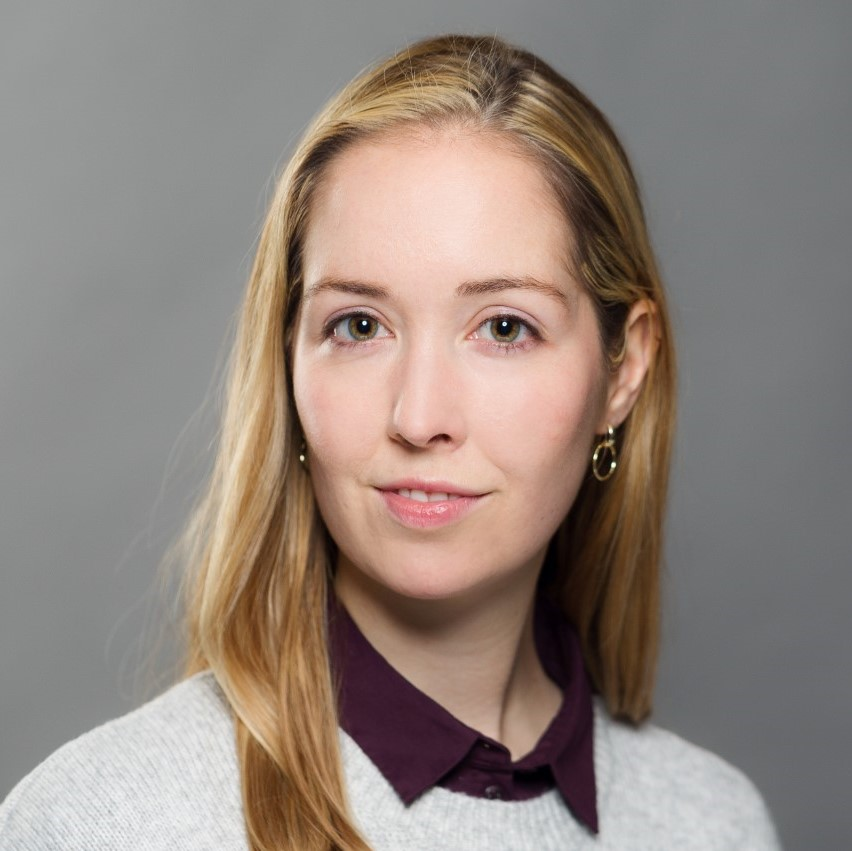
\includegraphics[width=0.65\textwidth]{aaf.jpg}\hfill\null

\noindent
\null\hfill%
\begin{tikzpicture}
    \clip (0,0) circle (1.75cm);
    \node at (0,0) {\includegraphics[width=3.5cm]{\imagePath}}; 
\end{tikzpicture}%
\hfill\null

\vspace*{1ex}
% Localized centering for the name
{\centering 
\LARGE \textbf{\MakeUppercase{\firstName\ \lastName}}\\
}


%\headleft{About Me}
\headleft[no-line]{About Me}
\parbox{1\textwidth}{
{\small
\justifying
\noindent Software Engineer with 5+ years of experience. Since the beginning of my career, I have contributed to diverse projects across industries like telecommunications, automotive, and energy, building applications from scratch, implementing new features, and finding solutions. Beyond my technical skills, I am flexible, communicative, and motivated to expand my knowledge, master new concepts and share knowledge. If there are any tools or technologies that I am not yet familiar with, I am committed to learn them.
}}


\headleft{Contact}
{\small
\begin{tabular}{@{}l@{\hspace{0.5em}}l}
\faEnvelope & \href{mailto:\emailAddress}{\emailAddress} \\[0.8ex]
\faPhone & \href{https://wa.me/\phoneNumber}{\phoneNumber} \\[0.8ex]
\faLinkedinSquare & \href{\linkedinUrl}{\linkedinName} \\[1ex]
\faGithub & \href{\githubUrl}{\githubName} \\[0.8ex]
\faHome & \href{https://\homepageUrl}{\homepageName} \\[0.8ex]
\end{tabular}
}


\headleft{Personal Information}
{\small
\begin{tabular}{@{}l@{\hspace{0.5em}}l@{}} % Align text with space between columns
\textbf{Citizenship:} & Swiss, German \\[0.8ex]
\textbf{Located in:}  & Freiburg (Germany) \\ 
                      & Les Houches (France) \\[0.8ex]
\textbf{Languages:}   & \\[0.4ex] % Empty space for separation
\end{tabular}

\begin{itemize}[leftmargin=1em]
    \item German (native language, C2)
    \item English (C1)
    \item Spanish (C1)
    \item French (B1)
\end{itemize}
}

\headleft{Technologies \& Tools}
{\small
\begin{itemize}[leftmargin=0.8em]
    \setlength{\itemsep}{0.5em}
    
    \item \textbf{Programming Languages}\\
    Python, TypeScript, JS, Java, C\#
    \item \textbf{Frontend}\\
     React, Vue, Angular, Redux, Material UI, Bootstrap, Tailwind CSS, HTML/CSS
    \item \textbf{Backend}\\
    Python Django, NodeJS, MongoDB, SQL
    \item \textbf{Testing}\\
    Java/Selenium, Cypress / Cucumber, Postman (API Testing), Jest
    \item \textbf{Agile Practices}\\
     Git, CI/CD, SCRUM, Jira, Confluence
\end{itemize}
}

\end{minipage}%
\kern0.09\textwidth\relax
}
\end{minipage}
\hskip2.5em
\begin{minipage}[t]{0.56\textwidth}
\setlength{\parskip}{0.8ex}

\vspace{2ex}

%%%%%%%%%%%%%%%%%%%%%%%%%%%%%%%%%%%%%%%%%%%%%%%%%%%%%%%
%                 RIGHT COLUMN                      %
%%%%%%%%%%%%%%%%%%%%%%%%%%%%%%%%%%%%%%%%%%%%%%%%%%%%%%%

\headright[no-line]{Experience}
%\headright{Experience}

\renewcommand{\labelitemi}{$\diamond$}

\experience{Software Engineer · IT Consultant}
    {Devoteam GmbH, Frankfurt, Germany · Remote}
    {February 2022 -- Now}

\begin{itemize}
    \item Development of web applications, leveraging cloud technologies, for data visualization with React, MaterialUI, with TypeScript or JavaScript, increasing user satisfaction through the implementation of new functionality.
 \item Transforming client requirements into technical solutions, collaborated in meetings to ensure alignment with stakeholder expectations
     \item Resolving bugs, validating urgent fixes, developing automated tests with Java/Selenium, Cypress, leading to a reduction in system downtime
    \item Implemented Git integration within GitLab CI/CD pipelines to optimize version control and automate deployment workflows.
    \item Contributed to an agile SCRUM environment using Git, Jira, and Confluence to manage tasks and document workflows.
\end{itemize}

\experience{System Analyst}
    {ELCA Informatique SA, Granada, Spain · Switzerland}  
    {Jan. 2021 -- Jan. 2022}

\begin{itemize}
    \item Automation of business-critical processes and implementation of new functionality in the company-wide production ERP system with Python.
    \item Creating and optimizing VBA scripts to generate business reports.
    \item Querying databases with SQL to ensure data accuracy and integrity.
    \item Conducted business analysis for new features, drafting user stories and acceptance criteria, and coordinating client meetings with stakeholders in Switzerland while collaborating within an international team comprising Spanish, German, and French-speaking colleagues.
\end{itemize}

\experience{Software Engineer (Internship)}
    {Intel Labs, Karlsruhe, Germany}  
    {Aug. 2019 -- Jan. 2020}

\begin{itemize}
   \item Automotive software development for an open-source simulator 
{\hypersetup{urlcolor=black}\href{https://carla.org/}{CARLA.org}} used for autonomous driving research.

    \item Developed traffic scenarios which describe traffic situations and vehicle behaviors like a lane change with Python.
    \item Debugging, testing, and implementing unsupported Parser features.
\end{itemize}

\experience{System Engineer (Internship)}
    {BMW M, Munich, Germany}  
    {Sep. 2018 -- Feb. 2019}
    
\begin{itemize}
    \item Developing a Windows desktop app with C\# to automatically translate bus communication protocols from LIN to CAN and vice versa.
    \item Antenna measurements during test drives in disguised prototype cars.
    \item Coordination of the annual tire change for vehicle fleets, including vehicle bookings, mechanic scheduling, and measurement/technical documentation of wheelbase parameters.
\end{itemize}

%%%%%%%%%% EDUCATION %%%%%%%%%%

\headright{Education}

\education{M. Sc. Electrical Engineering and Information Technology}
          {Karlsruhe Institute of Technology (KIT)}
          {2018 -- 2020}

\education{B. Sc. Electrical Engineering and Information Technology}
          {Karlsruhe Institute of Technology (KIT)}
          {2013 -- 2018}


%%%%%%%%%% CERTIFICATIONS %%%%%%%%%%
\headright{Certifications}

\begin{itemize}
\item \cert{2024}{Professional Python Programmer Level 1}{pythoninstitute.org}{https://verify.openedg.org/?id=gqtL.HUbN.Eshb}
\item \cert{2024}{ISTQB Certified Tester Foundation Level}{atsqa.org}{https://www.istqb.org/certifications/certified-tester-foundation-level-ctfl-v4-0/}
\item \cert{2023}{AWS Certified Cloud Practitioner}{Amazon}{https://www.credly.com/badges/d7c6436d-91aa-4124-a530-67f185f6f372/public_url}
\item \cert{2023}{Google Cloud Engineer}{Google}{https://google.accredible.com/d46ea4b1-ef6d-4510-a2ed-23ae1cf0a7e6}
\item \cert{2023}{Google Cloud Digital Leader}{Google}{https://www.credential.net/b68d248c-d7ac-4b19-9ee7-7bfecfccc8b2}
\item \cert{2022}{Professional Scrum Master I}{scrum.org}{https://www.scrum.org/user/1062623}
\end{itemize}



\end{minipage}

\end{document}
